\documentclass[sigconf]{acmart}

\usepackage{booktabs} % For formal tables
% \usepackage[pdf]{pstricks}
% \usepackage{graphicx}
% \usepackage{epstopdf}
\usepackage[update,prepend]{epstopdf}

\def\proof{\par{\it Proof}. \ignorespaces}
\def\endproof{\vbox{\hrule height0.6pt\hbox{%
   \vrule height1.3ex width0.6pt\hskip0.8ex
   \vrule width0.6pt}\hrule height0.6pt
  }}

\newtheorem{assumptions}{Assumptions}
\newtheorem{assumption}[assumptions]{Assumption}
\newcounter{subassumption}[assumptions]
\renewcommand{\thesubassumption}{(\textit{\roman{subassumption}})}
\makeatletter
\renewcommand{\p@subassumption}{\theassumption}% Counter prefix.
\makeatother
\newcommand{\assume}{
% Just like \item in a list, but for an assume
  \refstepcounter{subassumption}%
  \par\thesubassumption~\ignorespaces}



%% for enumerate (1) (2)...
\renewcommand\labelenumi{(\theenumi)}

\DeclareMathOperator{\tr}{tr}
\DeclareMathOperator{\sign}{sign}
\DeclareMathOperator*{\argmax}{arg\,max}
%****************
% Math Operators
%****************
\DeclareMathOperator{\aff}      {aff}
\DeclareMathOperator{\cl}       {cl}
\DeclareMathOperator{\cone}     {cone}
\DeclareMathOperator{\coni}     {coni}
\DeclareMathOperator{\conv}     {conv}
\DeclareMathOperator{\diag}     {diag}
\DeclareMathOperator{\dom}      {dom}
\DeclareMathOperator{\epi}      {epi}
\DeclareMathOperator{\inertia}  {inertia}
\DeclareMathOperator{\interior} {int}
\DeclareMathOperator{\linspan}  {span}
\DeclareMathOperator{\lin}      {lin}
\DeclareMathOperator{\minimize} {minimize}
\DeclareMathOperator{\Null}     {Null}
\DeclareMathOperator{\paraff}   {par}
\DeclareMathOperator{\proj}     {Proj}
\DeclareMathOperator{\Range}    {Range}
\DeclareMathOperator{\rank}     {rank}
\DeclareMathOperator{\recc}     {recc}
\DeclareMathOperator{\recf}     {recf}
\DeclareMathOperator{\ri}       {ri}
\DeclareMathOperator{\subjectto}{subject~to}
\DeclareMathOperator{\trace}    {trace}
% \DeclareMathOperator{\prox}{prox}

\newcommand{\LCal}{\mathcal{L}}
\newcommand{\ACal}{\mathcal{A}}
\newcommand{\BCal}{\mathcal{B}}
\newcommand{\CCal}{\mathcal{C}}
\newcommand{\DCal}{\mathcal{D}}
\newcommand{\NCal}{\mathcal{N}}
\newcommand{\ICal}{\mathcal{I}}
\newcommand{\JCal}{\mathcal{J}}
\newcommand{\FCal}{\mathcal{F}}
\newcommand{\UCal}{\mathcal{U}}
\newcommand{\PCal}{\mathcal{P}}
\newcommand{\RCal}{\mathcal{R}}
\newcommand{\WCal}{\mathcal{W}}
\newcommand{\XCal}{\mathcal{X}}
\newcommand{\onebf}{\mathbf{1}}
\newcommand{\zerobf}{\mathbf{0}}
%\newcommand{\shrink}{\mathrm{shrink}}
\newcommand{\shrink}{\mathcal{S}}
\newcommand{\sgn}{\mathrm{sgn}}
\newcommand{\mat}{\mathrm{mat}}
\newcommand{\Xvec}{\mathrm{vec}}
\newcommand{\SGN}{\mathrm{SGN}}
\newcommand{\Tr}{\mathbf{Tr}}
\newcommand{\dotX}[1]{\left \langle #1, X \right \rangle }
\newcommand{\dotCX}[2]{\left \langle #1, #2 \right \rangle }
\newcommand{\etal}{{et al. }}
\newcommand{\Diag}{\mbox{Diag}}
\newcommand{\oneotwomu}{\frac{1}{2\mu}}
\newcommand{\oneomu}{\frac{1}{\mu}}
\newcommand{\st}{\mbox{ s.t. }}
\newcommand{\prox}{\mbox{prox}}

\newcommand{\Acal}{{\cal A}}
\newcommand{\Bcal}{{\cal B}}
\newcommand{\Ccal}{{\cal C}}
\newcommand{\Dcal}{{\cal D}}
\newcommand{\Ecal}{{\cal E}}
\newcommand{\Fcal}{{\cal F}}
\newcommand{\Gcal}{{\cal G}}
\newcommand{\Hcal}{{\cal H}}
\newcommand{\Ical}{{\cal I}}
\newcommand{\Jcal}{{\cal J}}
\newcommand{\Kcal}{{\cal K}}
\newcommand{\Lcal}{{\cal L}}
\newcommand{\Mcal}{{\cal M}}
\newcommand{\Ncal}{{\cal N}}
\newcommand{\Ocal}{{\cal O}}
\newcommand{\Pcal}{{\cal P}}
\newcommand{\Qcal}{{\cal Q}}
\newcommand{\Rcal}{{\cal R}}
\newcommand{\Scal}{{\cal S}}
\newcommand{\Tcal}{{\cal T}}
\newcommand{\Ucal}{{\cal U}}
\newcommand{\Vcal}{{\cal V}}
\newcommand{\Wcal}{{\cal W}}
\newcommand{\Xcal}{{\cal X}}
\newcommand{\Ycal}{{\cal Y}}
\newcommand{\Zcal}{{\cal Z}}


% Shorthand commands for (uppercase) blackboard letters:
\newcommand{\Ambb}{\mathbb{A}}
\newcommand{\Bmbb}{\mathbb{B}}
\newcommand{\Cmbb}{\mathbb{C}}
\newcommand{\Dmbb}{\mathbb{D}}
\newcommand{\Embb}{\mathbb{E}}
\newcommand{\Fmbb}{\mathbb{F}}
\newcommand{\Gmbb}{\mathbb{G}}
\newcommand{\Hmbb}{\mathbb{H}}
\newcommand{\Imbb}{\mathbb{I}}
\newcommand{\Jmbb}{\mathbb{J}}
\newcommand{\Kmbb}{\mathbb{K}}
\newcommand{\Lmbb}{\mathbb{L}}
\newcommand{\Mmbb}{\mathbb{M}}
\newcommand{\Nmbb}{\mathbb{N}}
\newcommand{\Ombb}{\mathbb{O}}
\newcommand{\Pmbb}{\mathbb{P}}
\newcommand{\Qmbb}{\mathbb{Q}}
\newcommand{\Rmbb}{\mathbb{R}}
\newcommand{\Smbb}{\mathbb{S}}
\newcommand{\Tmbb}{\mathbb{T}}
\newcommand{\Umbb}{\mathbb{U}}
\newcommand{\Vmbb}{\mathbb{V}}
\newcommand{\Wmbb}{\mathbb{W}}
\newcommand{\Xmbb}{\mathbb{X}}
\newcommand{\Ymbb}{\mathbb{Y}}
\newcommand{\Zmbb}{\mathbb{Z}}


\newcommand{\half}{\frac{1}{2}}
\newcommand{\br}{\mathbb{R}}
\newcommand{\ntn}{{n \times n}}
\newcommand{\mtn}{{m \times n}}

\newcommand{\dx}[2]{\frac{d#1}{d #2}}
\newcommand{\dxf}[1]{\frac{d}{d #1}}
\newcommand{\ddx}[2]{\frac{d^2 #1}{d #2 ^2}}
\newcommand{\paruxf}[1]{\frac{\partial }{\partial #1}}
\newcommand{\parux}[2]{\frac{\partial #1}{\partial #2}}
\newcommand{\pparuxf}[1]{\frac{\partial^2 }{\partial #1 ^2}}
\newcommand{\pparux}[2]{\frac{\partial^2 #1}{\partial #2 ^2}}
\newcommand{\pparuxy}[3]{\frac{\partial^2 #1}{\partial #2 \partial #3}}
\newcommand{\pparuxyf}[2]{\frac{\partial^2 }{\partial #1 \partial #2}}
\newcommand{\laplapu}[1]{\triangle #1}
\newcommand{\lapu}[1]{\nabla #1}
\newcommand{\lapdiv}[2]{\nabla \cdot (#1 \nabla #2)}


% Copyright
%\setcopyright{none}
%\setcopyright{acmcopyright}
%\setcopyright{acmlicensed}
\setcopyright{rightsretained}
%\setcopyright{usgov}
%\setcopyright{usgovmixed}
%\setcopyright{cagov}
%\setcopyright{cagovmixed}


% DOI
\acmDOI{10.475/123_4}

% ISBN
\acmISBN{123-4567-24-567/08/06}

%Conference
\acmConference[WOODSTOCK'97]{ACM Woodstock conference}{July 1997}{El
  Paso, Texas USA} 
\acmYear{1997}
\copyrightyear{2016}

\acmPrice{15.00}


\begin{document}
\title{SIG Proceedings Paper in LaTeX Format}
\titlenote{Produces the permission block, and
  copyright information}
\subtitle{Extended Abstract}
\subtitlenote{The full version of the author's guide is available as
  \texttt{acmart.pdf} document}


% The default list of authors is too long for headers}
\renewcommand{\shortauthors}{B. Trovato et al.}


\begin{abstract}
This paper provides a sample of a \LaTeX\ document which conforms,
somewhat loosely, to the formatting guidelines for
ACM SIG Proceedings.\footnote{This is an abstract footnote}
\end{abstract}

%
% The code below should be generated by the tool at
% http://dl.acm.org/ccs.cfm
% Please copy and paste the code instead of the example below. 
%
% \begin{CCSXML}
% <ccs2012>
%  <concept>
%   <concept_id>10010520.10010553.10010562</concept_id>
%   <concept_desc>Computer systems organization~Embedded systems</concept_desc>
%   <concept_significance>500</concept_significance>
%  </concept>
%  <concept>
%   <concept_id>10010520.10010575.10010755</concept_id>
%   <concept_desc>Computer systems organization~Redundancy</concept_desc>
%   <concept_significance>300</concept_significance>
%  </concept>
%  <concept>
%   <concept_id>10010520.10010553.10010554</concept_id>
%   <concept_desc>Computer systems organization~Robotics</concept_desc>
%   <concept_significance>100</concept_significance>
%  </concept>
%  <concept>
%   <concept_id>10003033.10003083.10003095</concept_id>
%   <concept_desc>Networks~Network reliability</concept_desc>
%   <concept_significance>100</concept_significance>
%  </concept>
% </ccs2012>  
% \end{CCSXML}

% \ccsdesc[500]{Computer systems organization~Embedded systems}
% \ccsdesc[300]{Computer systems organization~Redundancy}
% \ccsdesc{Computer systems organization~Robotics}
% \ccsdesc[100]{Networks~Network reliability}


% \keywords{ACM proceedings, \LaTeX, text tagging}


\maketitle

\section{Introduction}
% @Author: Xiaocheng Tang
% @Date:   2017-05-11 22:03:41
% @Last Modified by:   Xiaocheng Tang
% @Last Modified time: 2017-05-11 22:03:48
% !TEX root = ./abstract.tex



\section{End to End Learning for Item Categorization} 
% !TEX root = ./abstract.tex
\paragraph{Category Taxonomy}
Multi-class classification with a targeted taxonomy structure among categories is often considered as hierarchical classification. In this case the targets are often understood as sets of categories with closely related categories grouped in the same set. A standard approach then is to decompose the problem into a sequence of multi-class classifications in a recursive top-down manner: 
first discriminate the subsets of categories at the top level of the hierarchy before going down the next level to discern the categories (or sets of categories) in those subsets. This process is repeated until reaching the bottom level.  
There are however two major shortcomings about the approach: 1. \emph{error propagation} where the mistakes made at the top-level will be carried over all the way to the leaf categories, and 2. \emph{data scarcity and imbalance} where as the category become more specific the less training data there is for that category. 

In this work we propose a more elegant and efficient approach with end-to-end learning from feature representation to multi-class classification. First of all, we simplify the problem by only considering the leaf categories in the taxonomy. In other words we flatten the hierarchy so that the problem becomes classic multi-classification. 
The trade-off is that while in the top-down approach the problem is decomposed into smaller subproblems each with only a few categories, now we consider 1000+ leaf categories all at once. We will see that this enables us to achieve a globally optimal solution in a sense that given an item a personalized total ranking can be learned among all leaf categories. This also present challenges to the problem due to the large scale output space. 

Knowledge sharing (cite) has been shown to be important in multi-task learning scenarios like this where tasks are closely related and knowledge gained from one task can be used to facilitate the training of another one. 
We will also see that knowledge sharing is now possible by solving a unified single problem whereas before each subproblem is trained independently. 

\begin{figure}
\label{fig:taxonomy}
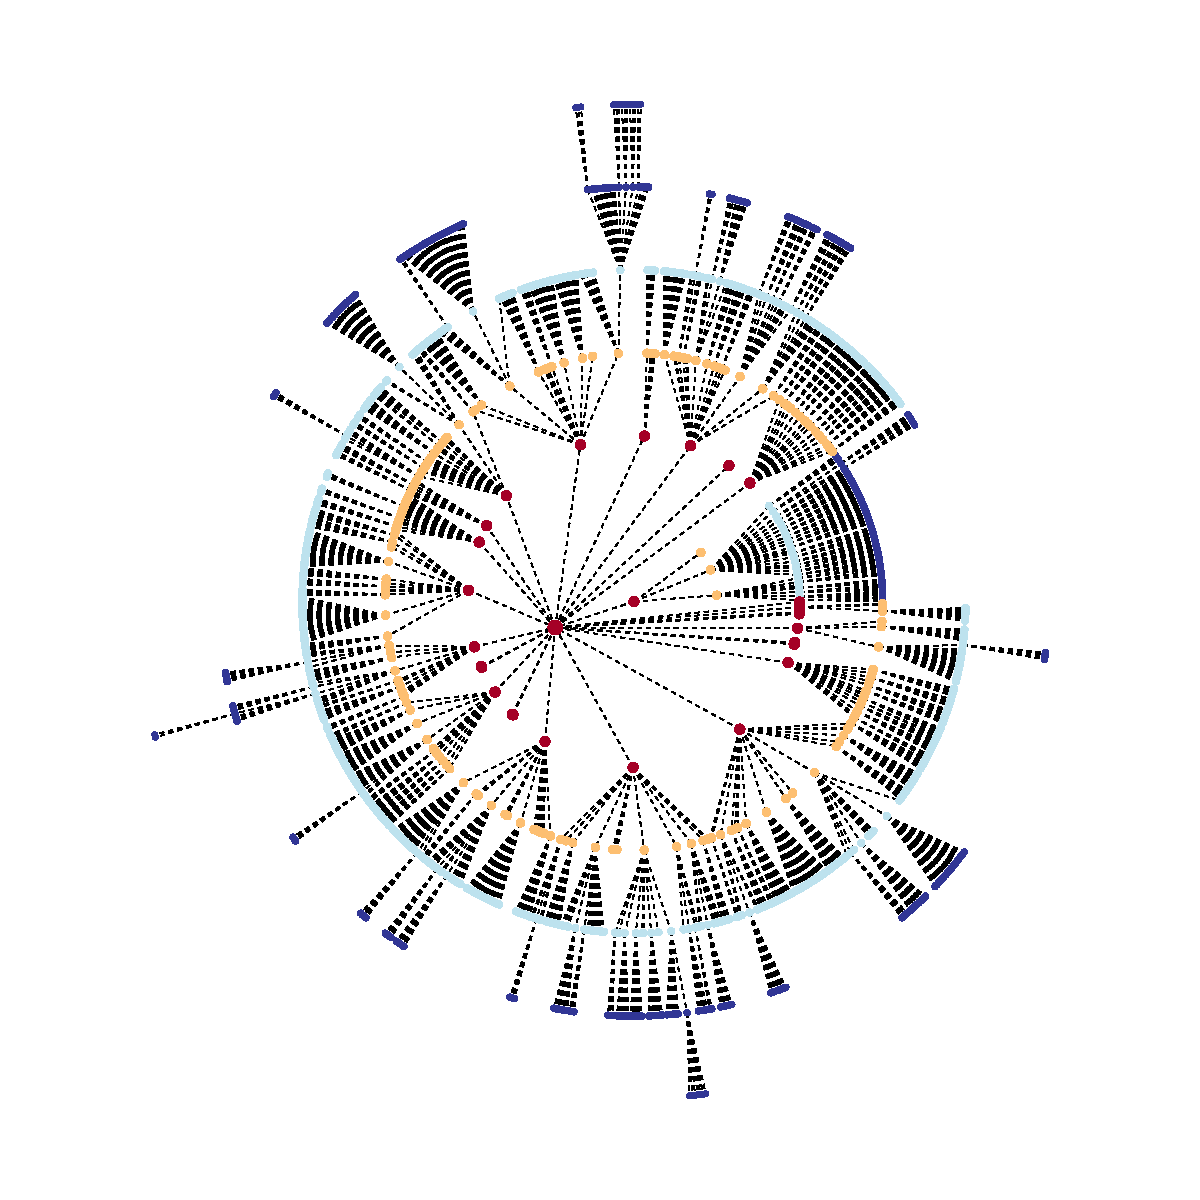
\includegraphics[width=0.5\textwidth]{resources/circular_tree.pdf}
\caption{An illustration of in-house taxonomy.}
\end{figure}

\paragraph{Negative Sampling With Log Loss}
A standard approach in multi-class classification is to maximize the log probability estimated using softmax. This can become computationally expensive when the output space is large due to the need to compute the normalization factor. In this work we make use of a more efficient alternative based on negative sampling (cite),
\begin{align}
\label{equ:obj}
    \JCal(\omega) = 
    - \log \sigma(f_{x, c_x}(\omega)) 
    - \sum_{i=1}^k E_{c_i \sim p_n(c)} \log \sigma(-f_{x, c_i}(\omega))
\end{align}
Here, the logit function $f_{x, c}(\omega)$ is parameterized by $\omega$ and applying the sigmoid function $\sigma(f_{x, c}(\omega))$ approximates the probability of the item $x \in \XCal$ being in the category $c \in \CCal$. 
By minimizing \eqref{equ:obj} we increase the probability of $x$ being in the ground truth category $c_x$ while decreasing the probability of $x$ in the wrong category sampled from the noise distribution $p_n(c)$. In this work we approximate it using $n_c / n$ which is the number of category $c$ in the training set divided by the total size of the training set. Note that \eqref{equ:obj} unlike Noise Contractive Estimation (cite) does not constitute an approximation to log probability of the full softmax. 
But it serves the purpose of classification where we only care about the top scores.

\paragraph{Joint Training of Item and Category Vector}
Here we discuss the specific structure we use for the logit function $f_{x, c}(\omega)$. The trainable parameters consist of the item matrix $U$ and a category matrix $V$. Each row in the item matrix corresponds to a feature we extract from the item description, and each row in the category matrix represents a particular category. The logits for all categories can then be obtained as,
\begin{align*}
    f_{x, \CCal}(U, V) = x^TUV^T
\end{align*}
Note that if letting $W = UV^T$ the above equation becomes $x^TW$ which is a standard form of multi-class classifier. By splitting $W$ into two matrices $U$ and $V$ we are essentially imposing a low-rank structure onto the classifier. This greatly reduces the number of learning parameters and has been widely used in recommendation system, multi-task learning, etc, to improve generalization.

In feature extraction we include both unigram and n-gram. We use all unigram and apply hashing tricks (cite) to n-gram, e.g., hashing each n-gram to a preset number of buckets. This has been shown to avoid overfitting and to improve system efficiency. In other words, if there are 1000 unique tokens and the bucket size is set to 500, then the dimension of $x$ will be 1000 + 500 = 1500 where each entry is 0 or 1 denoting whether the corresponding token or n-gram is present in the item description or not. In practice the size of the vector $x$ will be millions but very sparse. For efficient implementation we only store the indices of the non-zeros entries in $x$ and the matrix-vector multiplication between $x$ and $U$ takes only a loop through the non-zeros entries which are only the number of tokens in the item description. 

Now let us look at how we enable knowledge sharing in this context. Specifically, each task, or category in this case, corresponds to one row of the category matrix $V$, which captures the uniqueness of the task. The common knowledge shared by all task is reflected in the item matrix $U$. During training $U$ will be updated by examples regardless of which categories they belong to, while the rows in $V$ are only updated with the examples in the corresponding categories. In this way $U$ can help improve the accuracy of the category even though there are only a few training data in that category. This addresses the aforementioned \emph{data scarcity and imbalance} issues in the top-down approach.

\paragraph{Asynchronous SGD with Momentum}
The embedding matrices $U, V$ are trained using stochastic gradient descent with momentum and the updates are applied asynchronously in multiple threads. 
The major procedures are presented in Algorithm \ref{alg:asgd}. 
The main update rules are described in Line \ref{stp:asgd-update-begin}-\ref{stp:asgd-update-end}. 
Here $v_{c_x}$ denotes the vector representation of category $c_x$ and $u_i, i \in nnz(x)$ denotes the feature vector corresponding to the $i$th non-zero entry of $x$.
We will see that when the training dataset is highly sparse Algorithm \ref{alg:asgd} can be converted to a single-threaded implementation of block coordinate descent. In fact, consider two training examples $(x_1, c_1)$ and $(x_2, c_2)$ such that $nnz(x_1) \cap nnz(x_2) = \emptyset$ and that $c_1 \neq c_2$. According to Algorithm \ref{alg:asgd} $(x_1, c_1)$ and $(x_2, c_2)$ will result in update on $\omega_1 = (v_1, U_{nnz(x_1)})$ and $\omega_2 = (v_2, U_{nnz(x_2)})$, respectively. Note that $\omega_1$ and $\omega_2$ does not overlap because the categories and the non-zeros entries of training examples do not overlap. The computations of their partial derivatives are also independent of each other. 
Hence the update procedures in Line \ref{stp:asgd-update-begin}-\ref{stp:asgd-update-end} can happen simultaneously without the need for a lock.

Finally we make use of momentum in the update (Line \ref{stp:asgd-v-momentum} and \ref{stp:asgd-u-momentum}).

\begin{algorithm2e}[htb]
\caption{Asynchronous SGD With Momentum.}
\label{alg:asgd}
  Input: $\gamma \in (0, 1), \eta > 0, T > 0$, 
  the training set $\DCal \subset \XCal \times \CCal$ \\
  Initialize randomly the trainable parameters $U, V$ \\
  Initialize to zero the momentum parameters $\bar U, \bar V$ \\
  \For{each thread} {
    \For(\tcp*[h]{main iteration}) {$t=1,2,...,T$} {
	    sample $(x, c_x) \in \DCal$ \\
	    $\bar v_{c_x} \gets \gamma \bar v_{c_x} + \eta \nabla_{v_{c_x}} \JCal(U, V)$ \\
	    \label{stp:asgd-update-begin}
	    \label{stp:asgd-v-momentum}
	    $v_{c_x} \gets v_{c_x} - \bar v_{c_x}$ \\
	    \For{each $i \in nnz(x)$} {
	    	$\bar u_i \gets \gamma \bar u_i + \eta \nabla_{u_i} \JCal(U, V)$ \\
		    \label{stp:asgd-u-momentum}
	    	$u_i \gets u_i - \bar u_i$
	    }
	    \label{stp:asgd-update-end}
    }
  }
  Output: model parameters $U, V$
\end{algorithm2e}


























\section{Rule Integration Through Generative Modeling}
% @Author: Xiaocheng Tang
% @Date:   2017-05-11 22:01:21
% @Last Modified by:   Xiaocheng Tang
% @Last Modified time: 2017-05-21 00:23:37
% !TEX root = ./abstract.tex

In this work we utilize generative models to create new training labels and de-noise the data (\cite{Ratner2016}).
The model applies generative processes to labeling functions and learns their structural correlations and conflicts.
We incorporate numerous labeling functions as a supply of domain knowledge for weak supervision. Table (\ref{tab:numrules})
lists some of the categories and the number of rules associated with them. Labeling functions assign 1 if the product belongs

In this work we utilize generative models to create new training labels and de-noise the data (\cite{Ratner2016}).
The model applies generative processes to labeling functions $\lambda$ and learns their structural correlations and conflicts.
We incorporate numerous labeling functions as a supply of domain knowledge for weak supervision.

The generative model optimizes noise aware loss function and estimates probabilities $p(Label, \lambda)$,
where $Label$ is the category we want to predict, $\lambda = f(x)$ is a list of values assigned by labeling
functions $f$ to observation $x$, $\lambda : \chi \mapsto \{1, 0, -1\}^m$, where m is the number of labeling functions.
The values assigned by labeling functions are aggregated and serve as input to generative model.

Infered probabilies of the generative model are used to train another noise-aware end discriminative model which
predicts the ultimate categories.

% weak supervision, in which training labels are noisy and may be from
% multiple, potentially overlapping sources
% To address this, we model the labeling functions as a generative
% process, which lets us automatically de-noise the resulting training set by learning the accuracies of
% the labeling functions along with their correlation structure. In turn, we use this model of the training
% set to optimize a stochastic version of the loss function of the discriminative model that we desire to train.`'

\section{Data Pipeline}
% @Author: Xiaocheng Tang
% @Date:   2017-05-11 22:04:30
% @Last Modified by:   Xiaocheng Tang
% @Last Modified time: 2017-05-11 22:04:34
% !TEX root = ./abstract.tex



\section{Results}
% @Author: Xiaocheng Tang
% @Date:   2017-05-11 22:04:57
% @Last Modified by:   Xiaocheng Tang
% @Last Modified time: 2017-05-11 22:05:02
% !TEX root = ./abstract.tex



\section{Conclusions}
% @Author: Xiaocheng Tang
% @Date:   2017-05-11 22:05:25
% @Last Modified by:   Xiaocheng Tang
% @Last Modified time: 2017-05-11 22:05:34
% !TEX root = ./abstract.tex




\bibliographystyle{ACM-Reference-Format}
\bibliography{sigproc} 

\end{document}
